\subsection{Testaufbau}
Das Projekt wurde mit drei Nucleo-Boards als Nachbarn, welche alle mit unserem Code geflasht wurden, getestet. Die Baseboards wurden entsprechend in einer Kette zusammengesteckt. Für die Paketweiterleitung warenw jeweils Verbindungen vom Labyrinth zu drei Test-Nachbarn und zurück geschaltet. \\
Nach Beseitigung einiger Fehler wurde das Labyrinth einwandfrei mit den entsprechenden Ein- und Ausgängen generiert, gelöst und die Animation richtig abgespielt.

\subsection{Team 13 (Lego)}

\begin{figure}[H]
    \centering
    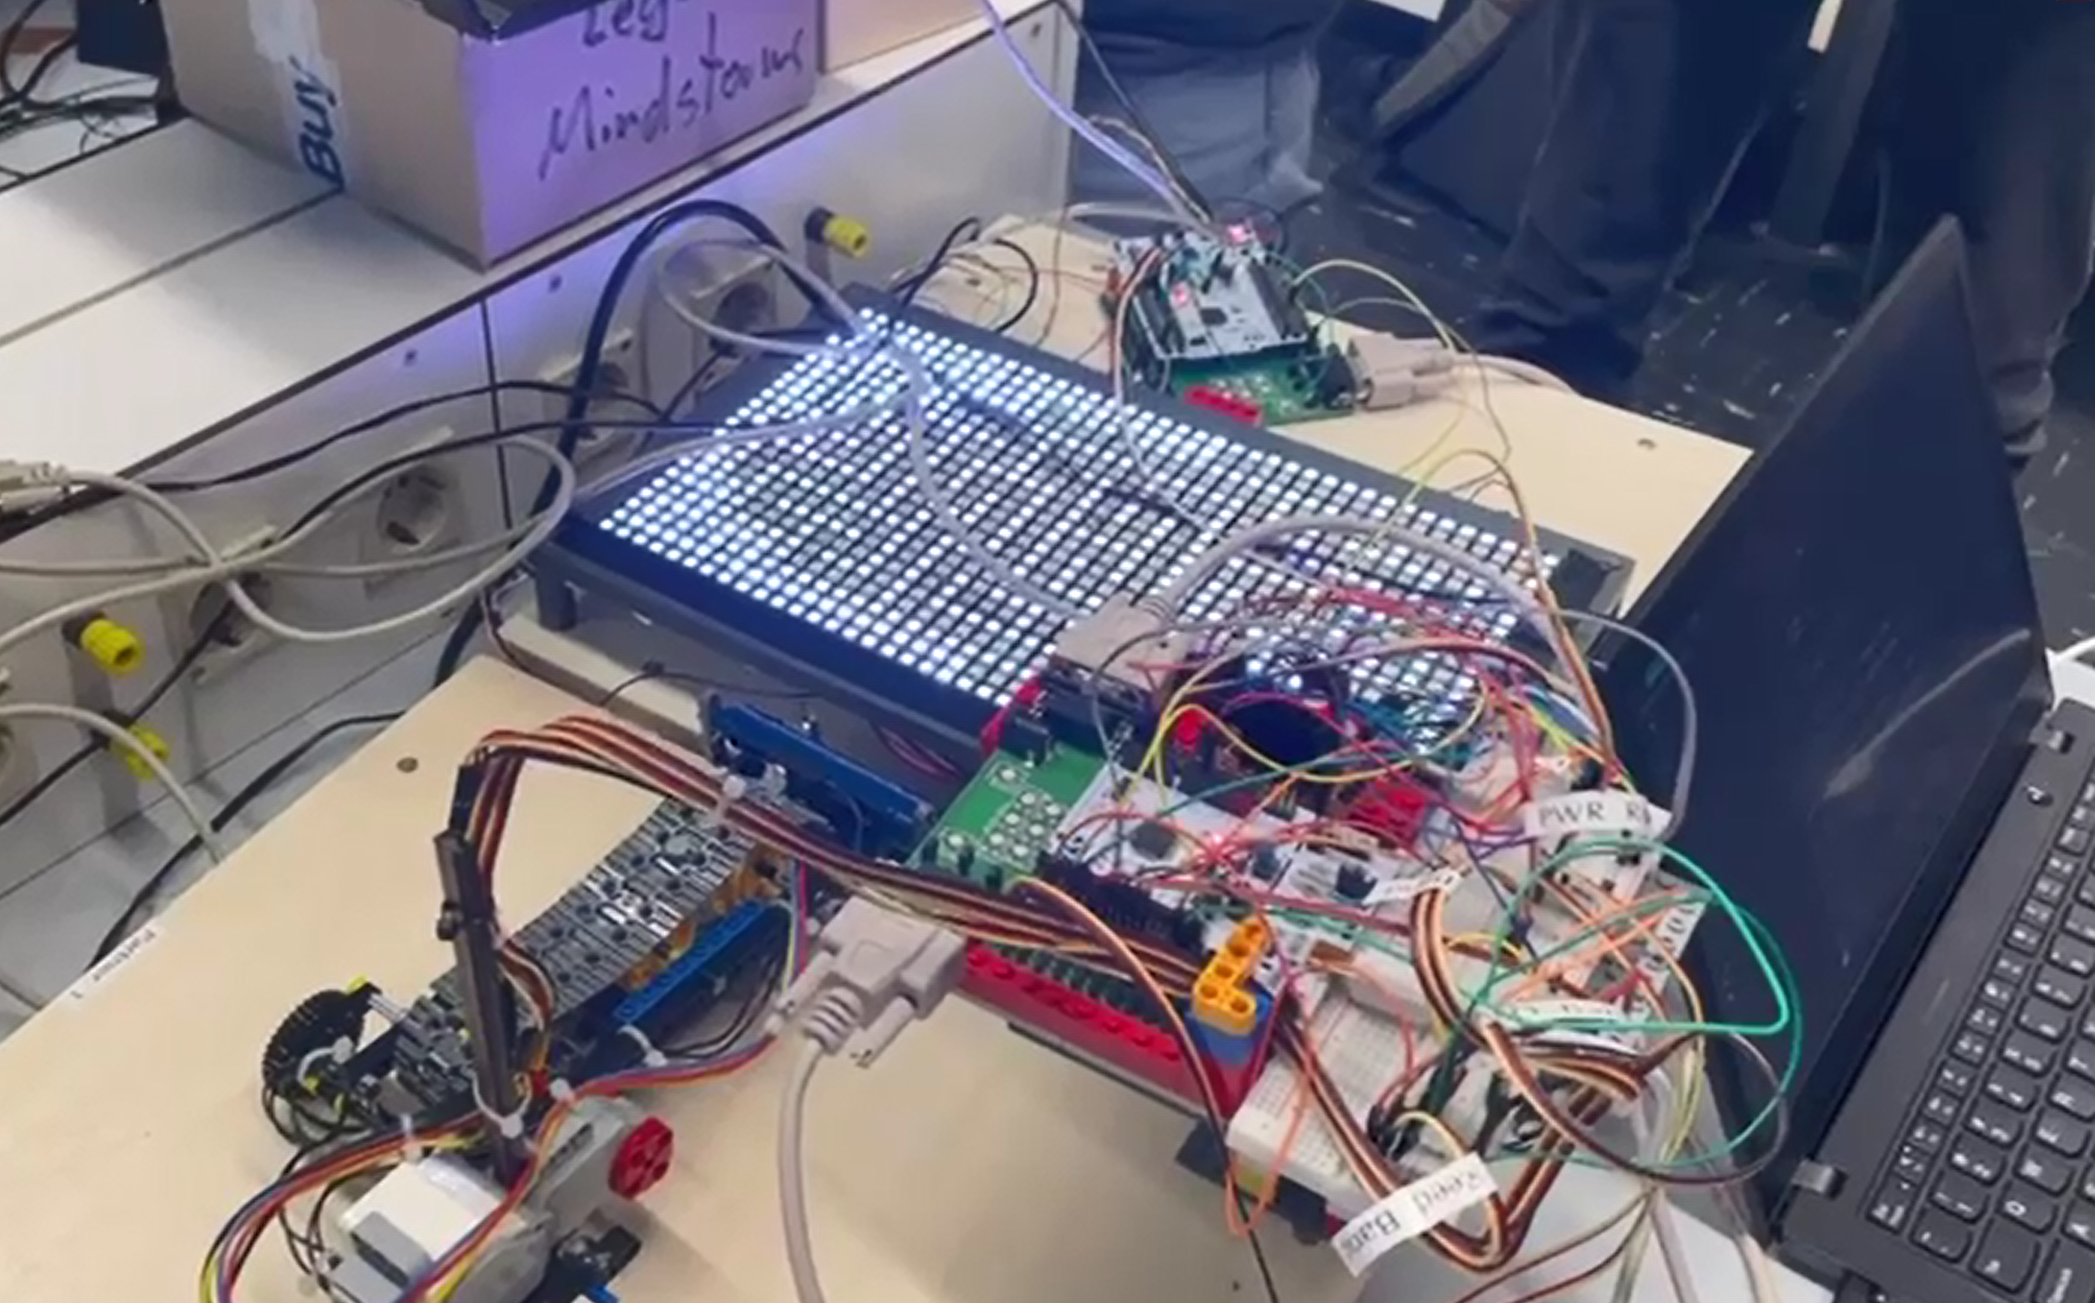
\includegraphics[page=1,width=0.78\textwidth]{images/Test_Team_13_cropped.PNG} 
    \caption{Test mit Team 13}
    \label{fig:Test_Team_13}
\end{figure}

Zunächst wurde die Interaktion mit dem System der Team 13 (Lego) getestet (Abb. \ref{fig:Test_Team_13}). Dazu wurden die Baseboards entsprechend zusammengesteckt. Der \enquote{Master} wurde dabei an das Baseboard unserer Teams angeschlossen, entsprechend wurde der \enquote{Chain End} Jumper beim Baseboard von Team 13 gesteckt. Im Testprogramm wurden zwei Routen konfiguriert:

\begin{lstlisting}[style=CBlank]
self.route[0] = [3,13] 
self.route[1] = [13,3]
\end{lstlisting}

\noindent Beide Routen funktionierten auf Anhieb einwandfrei:
\begin{itemize}
    \item das System fuhr zum korrekten Übergabepunkt
    \item das System wartete, bis das Paket vom Partner übergeben wurde
    \item das Paket wurde korrekt eingelagert - das System fuhr wieder zum richtigen Übergabepunkt und übergab das Paket erfolgreich an den Nachbarn
    \item der Nachbar nahm das Paket im richtigen Augenblick entgegen und lagerte es ein.
\end{itemize}
Obwohl die Paketweiterleitung funktionierte kam es beim Master-Programm zeitweise zur Meldung \texttt{\#\#\# ERROR \#\#\#}.

\subsection{Team 13 (Lego) und Team 12 (Roboterarm2)}

Anschließend wurden alle das Sytem mit den Aufbauten von Team 13 (Lego) und Team 12 (Roboterarm2) zusammengeschlossen. Folgende Routen wurden konfiguriert:

\begin{lstlisting}[style=CBlank]
self.route[0] = [3,13,12] 
self.route[1] = [12,13,3]
\end{lstlisting}

\noindent Hier funktionierte nur die erste Route. Ein Video dieses Tests ist hier hochgeladen \url{https://videos.portuus.de/w/9pmaQNVXYw2zNvjc7aKkho} Beim Empfang von Paketen von Team 12 kam es immer wieder zu Problemen, die nicht eindeutig zugeordnet werden konnten. 
Ebenfalls kam es in den anschließenden Testversuchen immer wieder zu Problemen bei der Übergabe an Team 12, entweder nahm der Roboterarm das Paket zu früh oder das Lego-Paketband nahm das Paket zu früh oder gar nicht entgegen. Mit Team 13 funktionierte auch in dieser Konstellation der Ablauf stehts einwandfrei. \\
Auch hier kam es beim Master-Programm zeitweise zur Meldung \texttt{\#\#\# ERROR \#\#\#} und es wurde mit zunehmender Paketanzahl instabiler.
